\section{Teori}

\subsection{Formål og bakgrunn}
Formålet med denne laboratorieøvelsen er å belyse prinsippene bak maskeanalyse og nodeanalyse. 
Det gjennomføres beregninger av gitte kretser ved bruk av begge metodene, for deretter å bekrefte resultatene eksperimentelt i laboratoriet. 
Videre skal øvelsen gi en praktisk forståelse av hvordan en Wheatstones målebru fungerer, og hvordan lineære potensiometre og temperaturavhengige motstander kan påvirke stabiliteten i broen.



\subsection{Teoretisk grunnlag}
Det teoretiske grunnlaget i både maske- og nodeanalyse kommer fra teorien bak ohms lov og Kirchhoffs lover.



\subsubsection{Ohms lov}
\label{paragraph:OhmsLov}

Ohms lov beskriver sammenhengen mellom spenning, strøm og motstand i en elektrisk krets. 
Den sier at strømmen gjennom en metallisk leder med konstant temperatur er proporsjonal med den elektriske potensialforskjellen (spenningen) over lederen \cite{wikipediaOhmsLov}. 
Den matematiske formuleringen av Ohms lov er:
\[
I = \frac{V}{R}, \qquad V = IR
\]
der $I$ er strømmen gjennom lederen, målt i ampere $[A]$, $V$ er potensialforskjellen (spenningen) over lederen, målt i volt $[V]$, og $R$ er motstanden (resistansen), målt i ohm $[\Omega]$. 

Figuren under viser en enkel krets der alle disse størrelsene inngår.

\begin{figure}[H]
\centering
\begin{circuitikz}[american voltages]
    \node[circle, draw=black, fill=none, thick, inner sep=2pt] (A) at (-1,2) {};
    \node[circle, fill=black, inner sep=1.2pt] (B) at (1,2) {};
    \node[circle, fill=black, inner sep=1.2pt] (C) at (1,-2) {};
    \node[circle, draw=black, fill=none, thick, inner sep=2pt] (D) at (-1,-2) {};

    \node at (-1, 1.6) {$+$};
    \node at (-1, -1.6) {$-$};
    \node at (-1, 0) {$V$};

    \draw (A) to[short, -, i^=$I$] (B);
    \draw (B) to[R=$R$] (C);
    \draw (C) to[short, -] (D);
    

\end{circuitikz}
\caption{Illustrasjon av Ohms lov i en enkel krets.}
\label{fig:ohmsLov}
\end{figure}

\paragraph{Anvendelse av Ohms lov i kretsanalyse}

Ohms lov utgjør grunnlaget for analyse av elektriske kretser. 
Ved å kombinere loven med Kirchhoffs spennings- og strømlover kan man bestemme ukjente strømmer og spenninger i komplekse nettverk. 
I praksis brukes Ohms lov til å beregne spenningen over, strømmen gjennom eller motstanden til et element når to av størrelsene er kjent. 
For eksempel kan loven brukes til å verifisere målte verdier fra laboratorieforsøk og kontrollere om komponentene oppfører seg lineært innenfor sitt spesifiserte område.



\subsubsection{Kirchhoffs lover}
Kirchhoffs lover er todelt og beskriver to forskjellige fenomen i kretsanalyse. Det er i hovedsak to regler for konservering av elektrisk ladning og elektrisk energi i strømkretser. Kirchhoffs lover er sentrale i kretselektronikk fordi det brukes for å finne forholdet mellom strøm og spenning. De to reglene refereres som \textbf{Kirchhoffs strømlov} og \textbf{Kirchhoffs spenningslov} \cite{wikipediaKirchhoffsLover}.

\paragraph{Kirchhoffs strømlov.}
\label{paragraph:KCL}
Denne loven beskriver prinsippet om konservering av elektrisk ladning i et forgreningspunkt: "I et forgreningspunkt er summen av alle inngående strømmer lik summen av alle utgående strømmer." \cite{wikipediaKirchhoffsLover}. Matematisk kan det beskrives følgende:
\[
\sum_{n=1}^{N}I_n=0, \qquad \text{forgrening med \textit{N} grener}
\]

\noindent
Figuren under viser et enkelt tilfelle av et forgreningspunkt. Her vil $i_2+i_3=i_1+i_4$.

\begin{figure}[H]
\centering
\begin{circuitikz}[american voltages]
    \node[circle, fill=black, inner sep=1.2pt] (A) at (0, 0) {};
    \node[circle, fill=black, inner sep=1.2pt] (B) at (0, 3) {};
    \node[circle, fill=black, inner sep=1.2pt] (C) at (3, 0) {};
    \node[circle, fill=black, inner sep=1.2pt] (D) at (0, -3) {};
    \node[circle, fill=black, inner sep=1.2pt] (E) at (-3, 0) {};


    \draw (A) to[R=$R_1$, i^=$i_1$] (B);
    \draw (C) to[short, -, i^=$i_2$] (A);
    \draw (D) to[R=$R_3$, i^=$i_3$] (A);
    \draw (A) to[short, -, i^=$i_4$] (E);
    

\end{circuitikz}
\caption{Illustrasjon av et forgreningspunkt.}
\label{fig:KCL}
\end{figure}

\paragraph{Kirchhoffs spenningslov.}
\label{paragraph:KVL}
Denne loven beskriver konservering av elektrisk energi og sier at: "Summen av alle elektriske potensialforskjeller (spenninger) i enhver lukket strømsløyfe er lik null" og kan matematisk uttrykkes som:
\[
\sum_{n=1}^{N} V_n = 0, \qquad \text{Sløyfe med \textit{N} forgreninger}
\]

\noindent
I kretser vil dette i praksis bety at positive potensialforskjeller over batterier må veies opp av negative potensialforskjeller over motstander eller andre komponenter. Figuren under viser et enkelt tilfelle av en sløyfe der $V_1 + V_2 + V_3 = V_4$.

\begin{figure}[H]
\centering
\begin{circuitikz}[american voltages]
    \node[circle, fill=black, inner sep=1.2pt] (A) at (-3, 2) {};
    \node[circle, fill=black, inner sep=1.2pt] (B) at (3, 2) {};
    \node[circle, fill=black, inner sep=1.2pt] (C) at (3, -2) {};
    \node[circle, fill=black, inner sep=1.2pt] (D) at (-3, -2) {};


    \draw (A) to[R=$R_1$] (B);
    \draw (B) to[R=$R_2$] (C);
    \draw (C) to[R=$R_3$] (D);

    \node at (0, 1.4) {$V_1$};
    \node at (2.3, 0) {$V_2$};
    \node at (0, -1.4) {$V_3$};

    \draw (A) to[V=$V_4$] (D);

    

\end{circuitikz}
\caption{Illustrasjon av en sløyfe.}
\label{fig:KVL}
\end{figure}



\subsubsection{Nodal analyse}

Prinsippet for nodeanalyse bygger direkte på Kirchhoffs strømlov \ref{paragraph:KCL} og Ohms lov \ref{paragraph:OhmsLov}. 
Ved hjelp av disse lovene kombinert sammen kan man sette opp ligninger for ukjente spenninger i en krets. 
Nodeanalyse baserer seg på at summen av alle strømmer som går \emph{inn} i et forgreningspunkt (node) er lik summen av alle strømmer som går \emph{ut} fra noden. 
Med Ohms lov kan dette uttrykkes som:
\[
\sum_{n=1}^{N} I_n = 0, \qquad I = \frac{V}{R}
\]

\begin{figure}[H]
\centering
\begin{circuitikz}
    % Node in the center
    \node[circle, fill=black, inner sep=1.2pt, label=above right:$V_A$] (A) at (0,0) {};
    
    % Define outer connection points
    \node[label=left:$V_1$]  (L) at (-3,0) {};
    \node[label=right:$V_2$] (R) at (3,0) {};
    \node[label=above:$V_3$] (T) at (0,2) {};
    \node[label=below:$V_4$] (D) at (0,-2) {};
    
    % Draw resistors to each branch
    \draw (L) to[R=$R_1$, i>_=$I_1$] (A);
    \draw (R) to[R=$R_2$, i>_=$I_2$] (A);
    \draw (T) to[R=$R_3$, i<_=$I_3$] (A);
    \draw (D) to[R=$R_4$, i<_=$I_4$] (A);
\end{circuitikz}
\caption{Node med fire grener. Strømmer $I_1$ og $I_3$ går inn i noden, mens $I_2$ og $I_4$ går ut.}
\label{fig:node_analysis}
\end{figure}

\noindent
Figur \ref{fig:node_analysis} viser et forgreningspunkt med to inngående strømmer $I_1$ og $I_2$, og to utgående strømmer $I_3$ og $I_4$. Kirchhoffs strømlov gir formel:
\begin{equation}
    I_1 + I_2 = I_3 + I_4
    \label{eq:node_analysis_base}
\end{equation}

\noindent
Vi kan utlede denne ligningen videre med å ta hensyn til spenningsforskjell over respektiv motstand. Spenningsforskjellen over en komponent kan uttrykes som forskjellen i spenning før og etter, $V_{ab} = V_a - V_b$. Det betyr at vi kan videreutforme ligning \ref{eq:node_analysis_base} som:
\[
\frac{V_1 - V_A}{R_1} + \frac{V_2 - V_A}{R_2} = \frac{V_A - V_3}{R_3} + \frac{V_A - V_4}{R_4} 
\]
\noindent
Denne fremgangsmåten kan utvides til flere noder for å etablere et lineært likningssystem som beskriver hele kretsen. 
Ved å løse disse likningene finner man de ukjente nodepotensialene og dermed alle strømmer i kretsen.




\subsubsection{Maskeanalyse}
Maskeanalyse bygger på prinsippene fra Kirchhoffs spenningslov \ref{paragraph:KVL} og Ohms lov \ref{paragraph:OhmsLov}. Vi kan derfor summere spenningen over en sløyfe med \textit{N} sløyfer slik:

\[
\sum_{n=1}^{N} V_n = 0, \qquad \sum_{n=1}^{N} I_nR_n = 0
\]

For å gjøre utføre maskeanalyse vil det være nødvendig å definere strømretninger innenfor de forskjellige sløyfene i en krets og ladninger ($+$ eller $-$) ved inngangsterminalene til komponenter. Under vil et eksempel for en to-sløyfe krets vise hvordan vi kan definere slike terminalladninger og strømretninger.


\begin{figure}[H]
\centering
\begin{circuitikz}[american voltages]

    % --- Noder ---
    \node[circle, fill=black, inner sep=1.2pt] (A) at (-5,2) {};
    \node[circle, fill=black, inner sep=1.2pt] (B) at (0,2) {};
    \node[circle, fill=black, inner sep=1.2pt] (C) at (5,2) {};
    \node[circle, fill=black, inner sep=1.2pt] (D) at (5,-2) {};
    \node[circle, fill=black, inner sep=1.2pt] (E) at (0,-2) {};
    \node[circle, fill=black, inner sep=1.2pt] (F) at (-5,-2) {};


    % --- Komponenter ---
    \draw (A) to[R=$R_1$,*-] (B);
    \draw (B) to[R=$R_2$,-*] (C);
    \draw (B) to[R=$R_3$,*-*] (E);

    \node at (-3.4, 2.3) {$+$};
    \node at (-1.6, 2.3) {$-$};

    \node at (1.6, 2.3) {$+$};
    \node at (3.4, 2.3) {$-$};

    \node at (0.3, 0.9) {$+$};
    \node at (0.3, -0.9) {$-$};

    \draw (A) to[V=$V_1$, label position=right, *-*] (F);
    \draw (D) to[V=$V_2$, label position=left, *-*] (C);

    \draw (F) to[short,*-*] (E);
    \draw (E) to[short,*-*] (D);


    % --- Maske-strømmer (nå sentrert og runde) ---
    % Venstre maske
    \draw[->, very thick, >=Stealth] (-2.5,0) ++(0.9,0) arc (0:-330:0.9);
    \node at (-2.5,0) {$I_1$};

    % Høyre maske
    \draw[->, very thick, >=Stealth] (2.5,0) ++(0.9,0) arc (0:-330:0.9);
    \node at (2.5,0) {$I_2$};

\end{circuitikz}
\caption{To-sløyfe krets for maskeanalyse med maskestrømmene $I_1$ og $I_2$ (med klokka).}
\label{fig:mesh_two_loops}
\end{figure}

\noindent
Ved å følge strømmene i sløyfene og addere hver spenning over hver komponent kan vi uttrykke et likingssystem. Det lineære likningssystemet for denne kretsen vil være:

\begin{align}
    -V_1 + R_1I_1 + R_3(I_1-I_2) &= 0 \\
    -V_2 - R_3(I_1-I_2) + R_2I_2 &= 0
\end{align}

For hvert spenningsledd i sløyfen vi summerer vil fortegnet bestemmes av inngående terminals fortegn. I tilfellet der to strømmsløyfer inngår i én resistanse, ($R_3$ i figur \ref{fig:mesh_two_loops}) vil man summere strømmene med henholdsvis fortegn i retning av terminalene pluss ($+$) til minus ($-$).




\subsection{Wheatstone-bro}
En Wheatstone-bro er en elektrisk krets som er brukt for å måle en ukjent motstand. Metoden for dette er ved å balansere beinene i brokretsen. I tillegg har denne elektriske kretsen en fordel med å kunne gi ekstremt nøyaktige målinger i kontrast til en spenningsdeler. Wheatstonebroa er oppfunnet av Samuel Hunter Christie i 1833, men var forbedret og kjentgjort av Charles Wheatstone i 1843. \cite{wikipediaWheatstoneBridge}

\paragraph{Kretsen. } Kretsen til en Wheatstone-bro består av 2 parallellkoblet par av resistorer i seriekobling. I tillegg er det en spenningskilde. Dermed får vi to noder vi kan måle spenningen mellom for vår interesse. Dermed ser kretsen slik ut.

\begin{figure}[H]
\centering
\begin{circuitikz}[american voltages]

    % Diamond corners
    \node[circle, fill=black, inner sep = 1.2pt] (T) at (2,  2) {};  % top
    \node[circle, fill=black, inner sep = 1.2pt, label=left:$A$] (L) at (0, 0) {};  % left
    \node[circle, fill=black, inner sep = 1.2pt, label=right:$B$] (R) at ( 4, 0) {};  % right
    \node[circle, fill=black, inner sep = 1.2pt] (B) at (2, -2) {};  % bottom

    \node[circle, fill=black, inner sep = 1.2pt] (a) at (-4, 3) {};
    \node[circle, fill=black, inner sep = 1.2pt] (b) at (2, 3) {};
    \node[circle, fill=black, inner sep = 1.2pt] (c) at (2, -3) {};
    \node[circle, fill=black, inner sep = 1.2pt] (d) at (-4, -3) {};

    % Sides (use R for resistors; use short for just an outline)
    \draw (T) to[R, l_=$R_1$] (L);
    \draw (T) to[R=$R_2$] (R);
    \draw (B) to[R=$R_3$] (L);
    \draw (B) to[R, l_=$R_4$] (R);

    \draw (a) to[short,*-*] (b);
    \draw (b) to[short,*-*] (T);
    \draw (B) to[short,*-*] (c);
    \draw (c) to[short,*-*] (d);
    \draw (a) to[V=$V_{in}$] (d);

    \draw (L) to[voltmeter=$V_{out}$] (R);

\end{circuitikz}
\caption{Wheatstone-bro}
\label{fig:wheatstone_bridge}
\end{figure}

\paragraph{Utledning av formel ved balansert bro.}
I tilfellet av en balansert bro kan vi bruke Kirchhoffs strømlov \ref{paragraph:KCL} og Kirchhoffs spenningslov \ref{paragraph:KVL} for å utlede en formel for $V_{out}$. Definerer vi en strøm $I_G$ som går fra $A$ til $B$ kan vi sette opp Kirchhoffs strømlov i node $A$ og $B$ henholdsvis:
\[
I_1 = I_G + I_3
\]
\[
I_2 + I_G = I_4
\]
\noindent
Deretter, ved bruk av Kirchhoffs spenningslov kan vi sette opp to strømsløyfer med klokka. I øvre sløyfe har vi $I_T$ og i nedre har vi $I_B$.
\[
-R_1(I_T) + R_2(I_T) - R_G(I_B - I_T) = 0
\]
\[
+ R_G(I_B - I_T) + R_4(I_B) - R_3(I_B) = 0
\]
Strømmen som går gjennom $R_G$ må være $0$ i en balansert bro. Som betyr at $I_B - I_T = 0$. Ligningsystemet kan skrives som:
\begin{align}
    R_2 \cdot I_T &= R_1 \cdot I_T \label{eq:l1_wheatstone} \\
    R_4 \cdot I_B &= R_3 \cdot I_B \label{eq:l2_wheatstone}
\end{align}

\noindent
Ligning \ref{eq:l1_wheatstone} deles på \ref{eq:l2_wheatstone} og vi får:

\[
R_4 = \frac{R_3 \cdot I_B \cdot R_2 \cdot I_T}{I_B \cdot R_1 \cdot I_T}
\]
\begin{equation}
    \frac{R_4}{R_2} = \frac{R_3}{R_1} \qquad \rightarrow \qquad \frac{R_1}{R_3} = \frac{R_2}{R_4}
    \label{eq:balansertWheatstoneBro}
\end{equation}


\noindent
\paragraph{Utledning av $V_{out}$ i balansert bro.}
Teorien om spenningsdeling \ref{paragraph:wikipediaWheatstoneBridge} sier at spenningen i node A og B i figur \ref{fig:wheatstone_bridge} kan skrives slik:
\[
V_A = V_{in} \left( \frac{R_3}{R_1+R_3} \right)
\]
\[
V_B = V_{in} \left( \frac{R_4}{R_2+R_4} \right)
\]
$V_{out}$ er definert som $V_A - V_B$:
\[
V_{out} = V_{in} \left( \frac{R_3}{R_1+R_3} \right) - V_{in} \left( \frac{R_4}{R_2+R_4} \right)
\]
\begin{equation}
V_{out} = V_{in} \left( \frac{R_3}{R_1+R_3} - \frac{R_4}{R_2+R_4} \right)
\label{eq:spenning_i_wheatstone}
\end{equation}

\noindent
Ligning \ref{eq:spenning_i_wheatstone} er den endelige utledningen av spenningspotensialforskjellen i en Wheatstone-bro.



\subsubsection{Spenningsdeling og balanserte kretser}
\label{subsec:spenningsdeling}

\begin{figure}[H]
\centering
\begin{circuitikz}[american voltages]
    \node [circle, fill=black, inner sep = 1.2pt, label=above:$V_{in}$] (A) at (-5, 0) {};
    \node [circle, fill=black, inner sep = 1.2pt] (B) at (0, 0) {};
    \node [circle, fill=black, inner sep = 1.2pt] (C) at (5, 0) {};

    \node [circle, fill=black, inner sep = 1.2pt, label=right:$V_{node}$] (D) at (0, -2) {};

    \draw (A) to[R=$R_L$] (B);
    \draw (B) to[R=$R_R$] (C);

    \draw (B) to[short, -] (D);
    \node[ground] (GND) at (C) {};

\end{circuitikz}
\caption{Spenningsdeler krets}
\label{fig:spenningsdeler}
\end{figure}

En ideell spenningsdeler med to seriemotstander $R_\mathrm{topp}$ og $R_\mathrm{bunn}$ tilført $V_{in}$ gir noden mellom dem spenningen
\[
V_\mathrm{node} = V_{in}\frac{R_R}{R_L+R_R}.
\]
Denne formelen brukes gjentatte ganger i kretsanalyse og er grunnlaget for utledningen av Wheatstone-broen. En Wheatstone-bro er \emph{balansert} når (ligning \ref{eq:balansertWheatstoneBro})
\[
\frac{R_1}{R_3}=\frac{R_2}{R_4},
\]
som er ekvivalent med at nodene har samme potensial, altså $V_{out}=0$. For ubalanse fås den kjente uttrykksformen (ligning \ref{eq:spenning_i_wheatstone})
\[
V_{out}=V_{in}\!\left(\frac{R_3}{R_1+R_3}-\frac{R_4}{R_2+R_4}\right).
\]
\paragraph{Følsomhet.}
Små endringer i én gren gir størst utslag når broen er nær balanse (bratteste helning rundt $V_{out}=0$), derfor er Wheatstone-broen velegnet til presis måling av små motstandsvariasjoner.

\subsubsection{Lineære potensiometre}
\label{subsec:potmeter}

Et lineært potensiometer har total motstand $R_P$ og en sleider (wiper) som deler motstanden i to: 
\[
R_\uparrow = \alpha R_P,\qquad R_\downarrow=(1-\alpha)R_P,\qquad \alpha\in[0,1].
\]
Potensiometret kan brukes på to måter:
\begin{enumerate}
  \item \textbf{Som spenningsdeler} (tre terminaler): noden ved sleideren får 
  \(
  V_\mathrm{wiper}=V_{in}\frac{R_\downarrow}{R_\uparrow+R_\downarrow}
  =V_{in}(1-\alpha).
  \)
  \item \textbf{Som variabel motstand} (rheostat, to terminaler): effektiv motstand er en funksjon av $\alpha$, typisk
  \(
  R(\alpha)=\alpha R_P
  \)
  (eller $(1-\alpha)R_P$ avhengig av hvilke terminaler som brukes).
\end{enumerate}

I denne rapporten modelleres potensiometre i Wheatstone-broen som \emph{variable motstander} $x$ i stedet for faste $R$ (rheostat-bruk). Setter vi for eksempel
\[
R_1=R,\quad R_2=x,\quad R_3=R,\quad R_4=x,
\]
får vi fra broformelen
\[
V_{out}(x)=V_{in}\!\left(\frac{R_3}{R_1+R_3}-\frac{R_4}{R_2+R_4}\right)
=V_{in}\!\left(\frac{R}{R+R}-\frac{x}{x+R}\right)
=V_{in}\frac{R-x}{R+x}.
\]
Skriver vi om med motsatt fortegn får vi varianten som brukes i plottet:
\[
V_{out}(x)=V_{in}\frac{x-R}{x+R}.
\]

\paragraph{Relevans for temperaturmåling.}
En temperaturavhengig motstand (PTC/NTC) oppfører seg som et potensiometer der \emph{temperatur} styrer $x$. Når én gren er referanse og den andre er sensor, gir en liten endring i $x(T)$ en målbar $\Delta V_{out}$ rundt balansepunktet.

\paragraph{Praktiske hensyn.}
\begin{itemize}
  \item \textbf{Linearitet}: lineær (B-taper) antas; logaritmisk (A-taper) er uegnet her.
  \item \textbf{Endestopp og wiper-motstand}: gir små, men merkbare feil nær $\alpha\approx0$ og $1$.
  \item \textbf{Lasting}: målte $V_{out}$ forutsetter høy inngangsimpedans på voltmeter/DAQ.
\end{itemize}




\subsection{Kretser}
\subsubsection{Krets 1}

\begin{figure}[H]
\centering
\begin{circuitikz}[american voltages]

    % Diamond corners
    \node[circle, fill=black, inner sep = 1.2pt, label=above left:$A$] (A) at (-5, 2) {};
    \node[circle, fill=black, inner sep = 1.2pt, label=above:$B$] (B) at (0, 2) {};
    \node[circle, fill=black, inner sep = 1.2pt, label=above right:$C$] (C) at ( 5, 2) {};
    \node[circle, fill=black, inner sep = 1.2pt] (F) at (-5, -2) {};
    \node[circle, fill=black, inner sep = 1.2pt] (E) at (0, -2) {};
    \node[circle, fill=black, inner sep = 1.2pt] (D) at (5, -2) {};

    \draw (A) to[V, a^=$V_1$, l_=$12\text{V}$, i>^=$I_{R1}$] (F);
    \draw (D) to[V, a^=$V_2$, l_=$12\text{V}$, i>^=$I_{R1}$] (C);

    \draw (A) to[R, a^=$R_1$, l_=$1.5\text{k}\Omega$, i>^=$I_{R1}$] (B);
    \draw (B) to[R, a^=$R_2$, l_=$1.5\text{k}\Omega$, i>^=$I_{R2}$] (C);
    \draw (B) to[R, a^=$R_3$, l_=$1.5\text{k}\Omega$, i>^=$I_{R3}$] (E);

    \draw (D) to[short,*-*] (E);
    \draw (E) to[short,*-*] (F);

    \draw (0, -2) node[ground]{}; 

\end{circuitikz}
\caption{Krets 1}
\label{fig:krets1}
\end{figure}

\paragraph{Maskeanalyse.} Ved å sette $I_1$ i venstre loop med klokka og $I_2$ i høyre loop med klokka, setter vi opp følgende likninger ved bruk av KVL:
\begin{equation}
    -12\text{V} + R_1(I_1) + R_3(I_1 - I_2) = 0
    \label{eq:maskeKrets1l1}
\end{equation}
\begin{equation}
    -12\text{V} - R_3(I_1 - I_2) + R_2(I_2) = 0
    \label{eq:maskeKrets1l2}
\end{equation}
Kjente verdier for $R_1$, $R_2$ og $R_3$ settes inn, og likningene løses for $I_1$ og $I_2$. Ligning \ref{eq:maskeKrets1l1} og \ref{eq:maskeKrets1l2} blir følgende:
\[
    3000\Omega(I_1) - 1500\Omega(I_2) = 12\text{V}
\]
\[
    3000\Omega(I_2) - 1500\Omega(I_1) = 12\text{V}
\]
Løsning av likningene gir:
\[
    I_1 = I_2 = 8\text{mA}
\]
\[
    I_{R1} = I_{R2} = 8\text{mA} \qquad I_{R3} = I_1 - I_2 = 0\text{mA}
\]
Spenningen for B uttrykkes ved å lese spenningsfallet fra A til B. Derfor blir spenningen i punkt A, B og C blir følgende: 
\[
    V_A = V_1 = 12\text{V}
\]
\[
    V_C = - V_2 = -12\text{V}
\]
\[
    V_B = V_A - R_1 \cdot I_{R1} = 12\text{V} - 1500\Omega \cdot 8\text{mA} = 0\text{V}
\]

\paragraph{Nodeanalyse.} \label{paragraph:nodeanalyse} For å beregne $I_{R1}$, $I_{R2}$ og $I_{R3}$ ved bruk av nodeanalyse trenger vi å sette opp Kirchhoffs strømlov (KCL) for node B i kretsen. Ved å sette bunn som felles jording ($0\text{V}$) setter vi opp følgende likning:
\[
    \frac{V_A-V_B}{R_1} = \frac{V_B-0\text{V}}{R_3} + \frac{V_B-V_C}{R_2}
\]
\begin{equation}
    \frac{12\text{V}-V_B}{1500\Omega} = \frac{V_B}{1500\Omega} + \frac{V_B+12\text{V}}{3000\Omega}
    \label{eq:KCLiB}
\end{equation}
\[
    V_B = 0\text{V}
\]
Ved å sette $V_B$ inn i likningene for $I_{R1}$, $I_{R2}$ og $I_{R3}$ får vi:
\begin{align}
    I_{R1} &= \frac{V_A - V_B}{R_1} = \frac{12\text{V} - 0\text{V}}{1500\Omega} = 8\text{mA} \\
    I_{R2} &= \frac{V_B - V_C}{R_2} = \frac{0\text{V} - (-12\text{V})}{1500\Omega} = 8\text{mA} \\
    I_{R3} &= \frac{V_B - 0\text{V}}{R_3} = \frac{0\text{V} - 0\text{V}}{1500\Omega} = 0\text{A} \\
\end{align}

\paragraph{Node B. }Spenningen i punkt B er $0\text{V}$. Dette er forventet da motstandene $R_1$ og $R_2$ har samme verdi, og spenningskilden på $12\text{V}$ er lik for begge sider av kretsen. Punkt B vil derfor være i midten av de to spenningskildene hvor den ene siden ha like stor positiv spenning som den andre siden har negativ spenning. Flyten av strøm vil derfor gå mellom spenningskildene og ingenting vil gå gjennom $R_3$. \\ Forholdet mellom resistorene er nødvendig for at spenningen i node B skal være $0\text{V}$. Det må være like stor spenning fra begge sider av noden for forsikre at strømmen flyter gjennom $R_1$ og $R_2$ uten å rømme gjennom $R_3$. For at spenning i node B skal være $0\text{V}$ må følgende forhold mellom resistorene være oppfylt:
\[
    R_1 = R_2, \qquad R_3 \; \epsilon \; \mathbb{R^+}
\]

\paragraph{Toleranse i resistansene.} En feilmargin på $\pm$1\% i resistansene vil påvirke spenningen i node B. For å finne det maksimale og minimale spenningsnivået i node B må vi se på hvordan spenningen oppfører seg over resistansene. Resistansene vil ha størrelseområde
\[
\begin{aligned}
    R_1 &\in [1485\Omega,\; 1515\Omega] \\
    R_2 &\in [1485\Omega,\; 1515\Omega] \\
    R_3 &\in [1485\Omega,\; 1515\Omega]
\end{aligned}
\]

Tilfelle med maksimum verdi i $V_B$ oppstår når spenningsfallet er minst over $R_1$ og størst over $R_2$. Dette er fordi spenningen over $R_1$ er positiv i forhold til node B, mens spenningen over $R_2$ er negativ i forhold til node B. Det vi også ønsker er å isolere noden mest mulig fra referansejording i bunn. Dermed konkluderer vi følgende:
\[
\begin{aligned}
    V_{B,\text{max}} &: \quad 
        R_1 = R_{1,\text{min}}, \;
        R_2 = R_{2,\text{max}}, \;
        R_3 = R_{3,\text{max}} \\[4pt]
    V_{B,\text{min}} &: \quad 
        R_1 = R_{1,\text{max}}, \;
        R_2 = R_{2,\text{min}}, \;
        R_3 = R_{3,\text{min}}
\end{aligned}
\]
Ved å sette inn verdiene i likningen for KCL i node B får vi to ligninger som kan løses for $V_{Bmax}$ og $V_{Bmin}$. i praksis blir dette maksimum og minimum verdi vi kan se i målinger. Resultatet skal ligge mellom disse to verdiene.
\[
    \frac{V_A-V_{Bmax}}{1485\Omega} = \frac{V_{Bmax}-0\text{V}}{1515\Omega} + \frac{V_{Bmax}+12\text{V}}{1500\Omega}
\]
\[
    \frac{V_A-V_{Bmin}}{1515\Omega} = \frac{V_{Bmin}-0\text{V}}{1485\Omega} + \frac{V_{Bmin}+12\text{V}}{1500\Omega}
\]
\begin{equation}
    V_{Bmax}=0.80\text{mV}, \qquad V_{Bmin}=-0.80\text{mV}
    \label{eq:VBminmax}
\end{equation}

\subsection{Krets 2}

\begin{figure}[H]
\centering
\begin{circuitikz}[american voltages]

    % Diamond corners
    \node[circle, fill=black, inner sep = 1.2pt, label=above left:$A$] (A) at (-5, 2) {};
    \node[circle, fill=black, inner sep = 1.2pt, label=above:$B$] (B) at (0, 2) {};
    \node[circle, fill=black, inner sep = 1.2pt, label=above right:$C$] (C) at ( 5, 2) {};
    \node[circle, fill=black, inner sep = 1.2pt] (F) at (-5, -2) {};
    \node[circle, fill=black, inner sep = 1.2pt] (E) at (0, -2) {};
    \node[circle, fill=black, inner sep = 1.2pt] (D) at (5, -2) {};

    \node[circle, fill=black, inner sep = 1.2pt] (TL) at (-5, 4) {};
    \node[circle, fill=black, inner sep = 1.2pt] (TR) at (5, 4) {};


    \draw (A) to[V, a^=$V_1$, l_=$12\text{V}$, i>^=$I_{R1}$] (F);
    \draw (D) to[V, a^=$V_2$, l_=$12\text{V}$, i>^=$I_{R1}$] (C);

    \draw (A) to[R, a^=$R_1$, l_=$1.5\text{k}\Omega$, i>^=$I_{R1}$] (B);
    \draw (B) to[R, a^=$R_2$, l_=$1.5\text{k}\Omega$, i>^=$I_{R2}$] (C);
    \draw (B) to[R, a^=$R_3$, l_=$1.5\text{k}\Omega$, i>^=$I_{R3}$] (E);

    \draw (D) to[short,*-*] (E);
    \draw (E) to[short,*-*] (F);

    \draw (TL) to[R, a^=$R_4$, l_=$3.9\text{k}\Omega$, i>^=$I_{R4}$] (TR);
    \draw (A) to[short,*-*] (TL);
    \draw (TR) to[short,*-*] (C);

    \draw (0, -2) node[ground]{}; 

\end{circuitikz}
\caption{Krets 2}
\label{fig:krets2}
\end{figure}





\subsubsection{Maskeanalyse.} Vi definerer strømmene i de tre loopene som $I_1$, $I_2$ og $I_3$, alle med klokka. Ved bruk av KVL setter vi opp følgende likninger:


\begin{align}
    -12\text{V} + 1500\Omega (I_1 - I_3) + 1500\Omega (I_1 - I_2) &= 0 \label{eq:loop1} \\
    3900\Omega \cdot I_3 - 1500\Omega (I_2 - I_3) - 1500\Omega (I_1 - I_3) &= 0 \label{eq:loop2} \\
    -12\text{V} - 1500\Omega (I_1 - I_2) + 1500\Omega (I_2 - I_3) &= 0 \label{eq:loop3}
\end{align}

Løsning av likningene \ref{eq:loop1}, \ref{eq:loop2} og \ref{eq:loop3} gir:

\[
I_1 = 14.15\text{mA}, \quad
I_2 = 14.15\text{mA}, \quad
I_3 = 6.15\text{mA}
\]

Strømmene $I_1$, $I_2$ og $I_3$ definerer $I_{R1}$, $I_{R2}$, $I_{R3}$, $I_{R4}$ og $I_{R5}$ som følger:
\[
I_{R1} = I_1 - I_3 = 8.0\text{mA}
\]
\[
I_{R2} = I_2 - I_3 = 8.0\text{mA}
\]
\[
I_{R3} = I_1 - I_2 = 0\text{A}
\]
\[
I_{R4} = I_3 = 6.15\text{mA}
\]

\paragraph{Spenningene i nodene A, B og C.} Spenningene kan uttrykkes på samme måte som i ligning \ref{eq:KCLiB} under \ref{paragraph:nodeanalyse}. Ettersom at grenen fra node A til C vil ikke utgjøre en forskjell på $V_A$ og $V_C$ sammenlignet med krets 1, vil spenningene i nodene A, B og C være de samme som i krets 1:
\[
V_A = 12\text{V}, \quad V_B = 0\text{V}, \quad V_C = -12\text{V}
\]

\subsection{Krets 3}

\begin{figure}[H]
\centering
\begin{circuitikz}[american voltages]

    \node[circle, fill=black, inner sep = 1.2pt] (A) at (-6,  -2) {};
    \node[circle, fill=black, inner sep = 1.2pt] (B) at (-6,  2) {};
    \node[circle, fill=black, inner sep = 1.2pt] (C) at (-5,  2) {};
    \node[circle, fill=black, inner sep = 1.2pt] (D) at (-5,  3) {};
    \node[circle, fill=black, inner sep = 1.2pt] (E) at (-5,  1) {};

    \node[circle, fill=black, inner sep = 1.2pt, label=above:$1$] (F) at (0,  3) {};
    \node[circle, fill=black, inner sep = 1.2pt, label=below:$2$] (G) at (0,  1) {};

    \node[circle, fill=black, inner sep = 1.2pt] (H) at (5,  2) {};
    \node[circle, fill=black, inner sep = 1.2pt] (I) at (5,  3) {};
    \node[circle, fill=black, inner sep = 1.2pt] (J) at (5,  1) {};
    \node[circle, fill=black, inner sep = 1.2pt] (K) at (6,  2) {};
    \node[circle, fill=black, inner sep = 1.2pt] (L) at (6,  -2) {};

    \draw (B) to[V, a^=$V_{in}$, l_=$12\text{V}$, i>^=$I_{R1}$] (A);
    \draw (K) to[short,*-*] (L);
    \draw (F) to[voltmeter=$V_{out}$] (G);

    \draw (A) node[ground]{};
    \draw (L) node[ground]{};
    \draw (B) to[short,*-*] (C);
    \draw (H) to[short,*-*] (K);

    \draw (C) to[short,*-*] (D);
    \draw (C) to[short,*-*] (E);

    \draw (H) to[short,*-*] (I);
    \draw (H) to[short,*-*] (J);

    \draw (D) to[R=$R_5$] (F);
    \draw (E) to[R=$R_7$] (G);

    \draw (F) to[R=$R_6$] (I);
    \draw (G) to[R=$R_8$] (J);



\end{circuitikz}
\caption{Wheatstone-bro}
\label{fig:krets3}
\end{figure}



Ligningen for spenningen i Wheatstone-broen er gitt som:
\begin{equation}
    V_{out} = V_{in} \cdot  \left(\frac{R_8}{R_7 + R_8} - \frac{R_6}{R_5 + R_6}\right)
    \label{eq:wheatstoneKrets3}
\end{equation}
Der $V_{out}$ er spenning mellom node 1 og 2 i broen. Når broen er balansert, vil $V_{out} = 0\text{V}$. Dette skjer når følgende forhold er oppfylt:
\[
\frac{R_8}{R_7 + R_8} = \frac{R_6}{R_5 + R_6}
\]
\[
R_5 = R_6 = R_7 = R_8
\]
\paragraph{Lineære potensiometre.} Vi undersøker hvordan temperatur kan måles ved hjelp av et resistivt måleprinsipp basert på temperaturavhengige motstander (PTC-motstander). Vi kan simulere slike motstandere med bruk av lineære potensiometre. En lineær potensiometer har en motstandsverdi som er proporsjonal med hvor mye av potensiometret som er vridd. Ved å sette opp en Wheatstone-bro med to lineære potensiometre, kan vi simulere en temperaturmåling. Når den ene potensiometren representerer en referansetemperatur og den andre representerer den målte temperaturen, vil broen være balansert ved referansetemperaturen. Når temperaturen endres, vil motstandsverdien i den målte potensiometren endres, noe som fører til en ubalanse i broen og dermed en målbar spenning $V_{out}$. \\ For å oppnå høyest mulig potensialforskjell mellom node 1 og 2 gjennom måling av $V_{out}$, bør potensiometerne plasseres slik at ligning \ref{eq:wheatstoneKrets3} kan få høyest mulig verdi. Plasserer vi begge potensiometerne før målenodene blir det fortsatt balanse. Derfor må de plasseres diagonalt i broen for å oppnå størst $|V_{out}|$. Vi bytter derfor ut $R_5$ og $R_8$ med potensiometre. Ligningen kan skrives følgende:
\[
V_{out} = V_{in} \cdot  \left(\frac{R_8}{R_7 + R_8} - \frac{R_6}{R_5 + R_6}\right), \qquad R_5 = R_6 = R_7 = R_8
\]
\[
V_{out}(x_{pot}) = V_{in} \cdot  \left(\frac{x_{pot}}{R + x_{pot}} - \frac{R}{x_{pot} + R}\right)
\]
\[
V_{out}(x_{pot}) = V_{in} \cdot  \left(\frac{x_{pot} - R}{R + x_{pot}} \right)
\]
\noindent
$V_{out}$ er nå en funksjon for $x_{pot}$ og vi kan plotte den.



\begin{figure}[H]
\centering
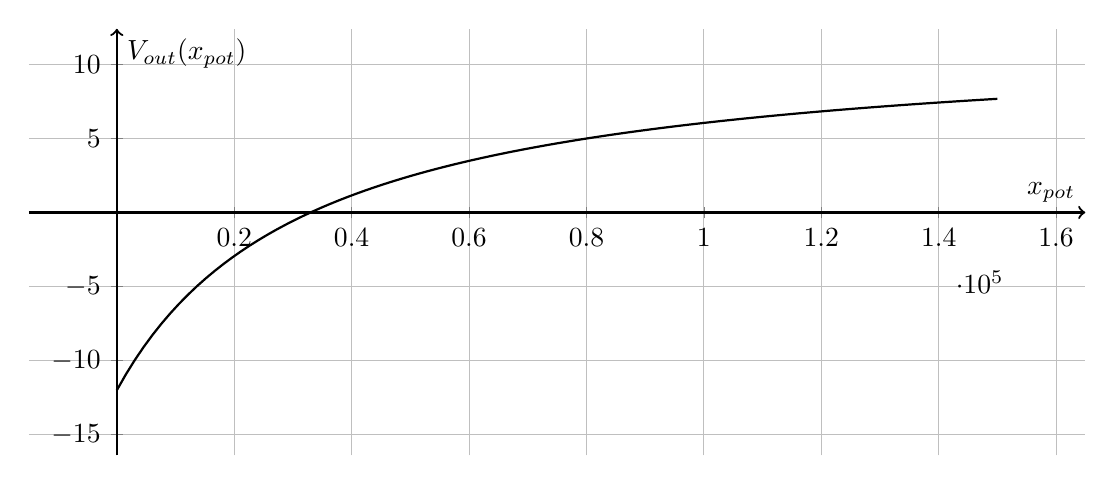
\begin{tikzpicture}
  \begin{axis}[
    xlabel=$x_{pot}$, 
    ylabel=$V_{out}(x_{pot})$,
    height=7cm,
    width=15cm,
    grid=both, 
    thick, 
    domain=0:150000, 
    samples=100, 
    ymin=-14, ymax = 10,
    axis lines=middle,           % move axes to the center (nice visual)
    axis line style={->},        % add arrows
    enlargelimits,               % small margin
  ]
    \addplot[black] {12 * ((x - 33000) / (x + 33000))};
  \end{axis}
\end{tikzpicture}
\caption{Graf}
\label{fig:wheatstone-graph}
\end{figure}

\vspace{1em}
\noindent
Grafens ekstremalpunkter i intervallet $x_{pot} \in [0, 100\text{k}\Omega]$ vil fortelle oss hva vi kan måle $V_{out}$ sin laveste og høyeste verdi vil være. Siden grafen oppfører seg som $V_{out}(s) < V_{out}(s + \Delta s)$ i intervallet $[0, 10^5]$ er den strengt økende og vi vil garantert finne dens laveste verdi i $x_{pot} = 0$ og høyest verdi i $x_{pot} = 10^5$. Dermed løser vi for det som:
\begin{align}
V_{out}(0) &= -12\text{V} \\
V_{out}(10^5) &= 6.05\text{V}
\end{align}